%  !TeX  root  =  user_guide.tex  
\section{L'extension Géoréférencer}

%The Georeferencer Plugin is a tool for generating world files for rasters.
%It allows you to reference rasters to geographic or projected coordinate systems by creating a 
%world file, or by transforming the raster to a new coordinate system. The basic approach to georeferencing a raster is to locate points on the raster for which you can accurately determine their coordinates. The source of the coordinates can be:

L'extension de géoréférencement est un outil permettant de renseigner les coordonnées des rasters en générant les fichiers "world" (fichiers de référence indiquant le système géographique ou projeté à employer) ou de les transformer dans un nouveau système. L'approche initiale pour géoréferencer une image est de localiser des points sur le raster dont vous pouvez déterminer les coordonnées. La source de ces coordonnées peut être :

%\begin{enumerate}
%\item The raster itself, sometimes coordinates are literally `written' on the raster. 
%In this case you can enter the coordinates manually.
%\item Other georeferenced data, this can be either vector or raster data that contain the same objects/features that you have on the raster that you want to georeference. In this case you can enter the coordinates by clicking on the reference dataset loaded in QGIS map canvas.
%\end{enumerate}

\begin{enumerate}
\item par le raster lui-même, quelquefois les coordonnées sont littéralement écrites (p. ex., les graticules). Dans ce cas, vous pouvez les saisir manuellement.
\item par des données déjà géoréférencées, cela peut être des données vecteurs ou rasters qui contient les mêmes objets/entités que le raster que vous désirer géoréférencer. Dans ce cas, il vous faudra renseigner les coordonnées en cliquant les données de référence qui auront été chargées dans la carte principale de QGIS.
\end{enumerate}

%The usual procedure for georeferencing an image involves selecting multiple points on the raster, 
%specifying their coordinates, and choosing a relevant transformation type. Based on the input parameters and data, the plugin will compute the world file parameters. The more coordinates you provide, the better the result will be.

La procédure standard pour lé géoréférencement d'une image implique la sélection de plusieurs points sur le raster, en spécifiant leurs coordonnées et en choisissant la transformation appropriée. En se basant sur les paramètres rentrés et les données, l'extension calculera les paramètres du fichier "world". Plus il y a de coordonnées fournies, meilleur sera le résultat.

%The first step is to start QGIS and load the Georeferencer Plugin (see Section 
%\ref{sec:load_core_plugin}) and click on the \toolbtntwo{georeferencer}{Georeferencer} 
%icon which appears in the QGIS toolbar menu. The Georeferencer Plugin dialog appears as 
%shown in Figure \ref{fig:georefplugin}.

La première étape est de lancer QGIS puis de charger l'extension (voir la section \ref{sec:load_core_plugin}) pour enfin cliquer sur l'icône \toolbtntwo{georeferencer}{Géoreferencer} qui apparaît dans la barre d'outils de QGIS. La fenêtre de géoréférencement se présente sous la forme montrée dans la figure \ref{fig:georefplugin}.
 
%For this example, we are using a topo sheet of South Dakota from SDGS. It can later be visualized 
%together with the data from the GRASS spearfish60 location. You can download the topo sheet here: 
%\url{http://grass.osgeo.org/sampledata/spearfish\_toposheet.tar.gz}

En guise d'exemple, nous allons utiliser un fichier world issu d'une carte topographique du Dakota du Sud publiée par le SDGS.
Elle pourra par la suite être affichée avec les données du secteur GRASS spearfish60. Cette carte topographique peut être téléchargée à l'adresse suivante : \url{http://grass.osgeo.org/sampledata/spearfish\_toposheet.tar.gz}

%\begin{figure}[ht]
%\begin{center}
%  \caption{Georeferencer Plugin Dialog \nixcaption}\label{fig:georefplugin}\smallskip
%  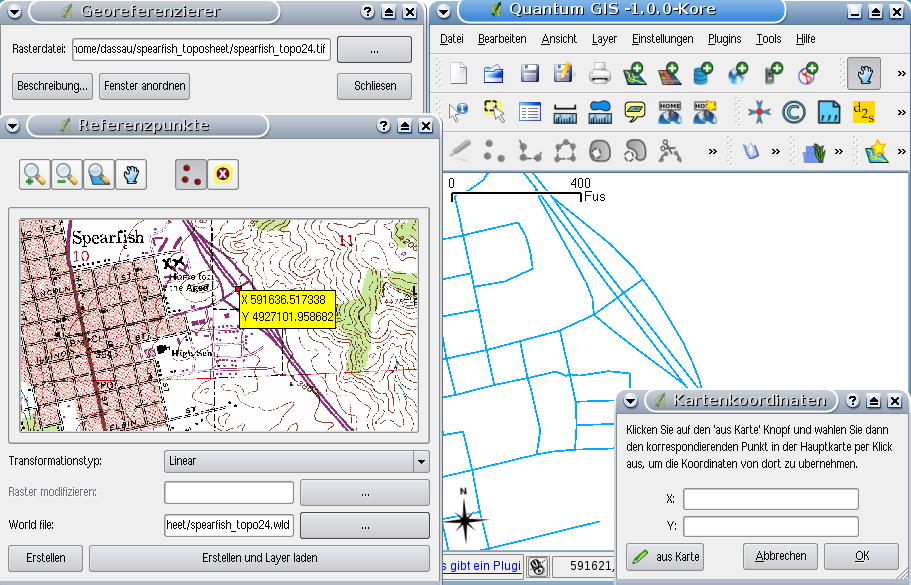
\includegraphics[clip=true, width=12cm]{georefplugin}
%\end{center}
%\end{figure}

\begin{figure}[ht]
\begin{center}
  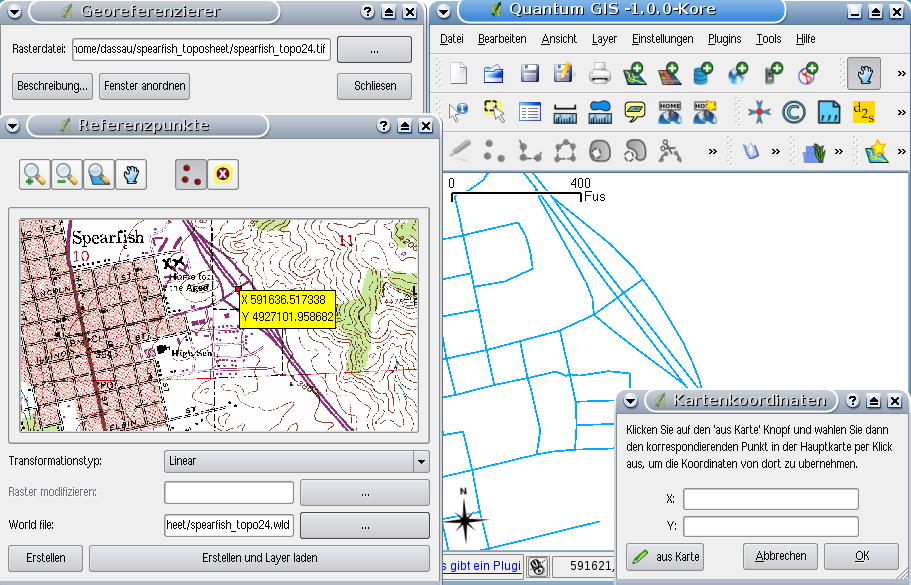
\includegraphics[clip=true, width=10cm]{georefplugin}
  \caption{Fenêtre de l'extension de géoréférencement \nixcaption}\label{fig:georefplugin}
\end{center}
\end{figure}

%\minisec{Entering ground control points (GCPs)}\label{georeferencer_entering}
\minisec{Saisir des points de contrôles (GCP)}\label{georeferencer_entering}

%\begin{enumerate}
%\item To start georeferencing an unreferenced raster, we must load it using the \browsebutton browse button. The raster will show up in the main working area of the dialog. Once the raster is loaded, we can start to enter reference points.
\begin{enumerate}
\item Pour commencer le géoréférencement d'un raster To start georeferencing an unreferenced raster, we must load it using the \browsebutton browse, nous devons le charger via le bouton \browsebutton. Le raster apparaît alors dans la surface principale de travail de la fenêtre. Une fois qu'il est chargé, nous pouvons commencez à entrer des points de coordonnés.

%\item Using the \toolbtntwo{mActionCapturePoint}{Add Point} button, add points to the main working area and enter their coordinates (See Figure \ref{fig:choose_points}). For this procedure you have two options:
\item En utilisant le bouton \toolbtntwo{mActionCapturePoint}{Ajouter des Points}, ajouter par un clic des points dans la surface de travail et saisissez leurs coordonnées (voir figure \ref{fig:choose_points}). Pour ce faire, il y a deux manières de procéder :

%\begin{enumerate}
%\item Click on a point in the raster map and enter the X and Y coordinates manually
%\item Click on a point in the raster map and choose the button \toolbtntwo{pencil}{from map canvas} to add the X and Y coordinates with the help of a georeferenced map already loaded in QGIS.
%\end{enumerate}
%\item Continue entering points. You should have at least 4 points, and the more coordinates you can provide, the better the result will be. There are additional tools on the plugin dialog to zoom and pan the working area in order to locate a relevant set of GCP points.
%\end{enumerate}

\begin{enumerate}
\item En cliquant en un point de la carte raster et entrant les coordonnées X et Y manuellement
\item En cliquant en un point de la carte raster puis sur le bouton \button{from map canvas} pour ajouter les coordonnées X et Y à l'aide d'une carte géoréférencée déjà chargée dans QGIS.
\end{enumerate}
\item Continuez de rentrer des points jusqu'à en avoir au moins 4. Des outils additionnels situés dans la partie supérieure de cette fenêtre permettent de zoomer et de se déplacer dans l'espace de travail.
\end{enumerate}

%%\begin{figure}[ht]
%\begin{center}
%  \caption{Add points to the raster image \nixcaption}\label{fig:choose_points}\smallskip
%  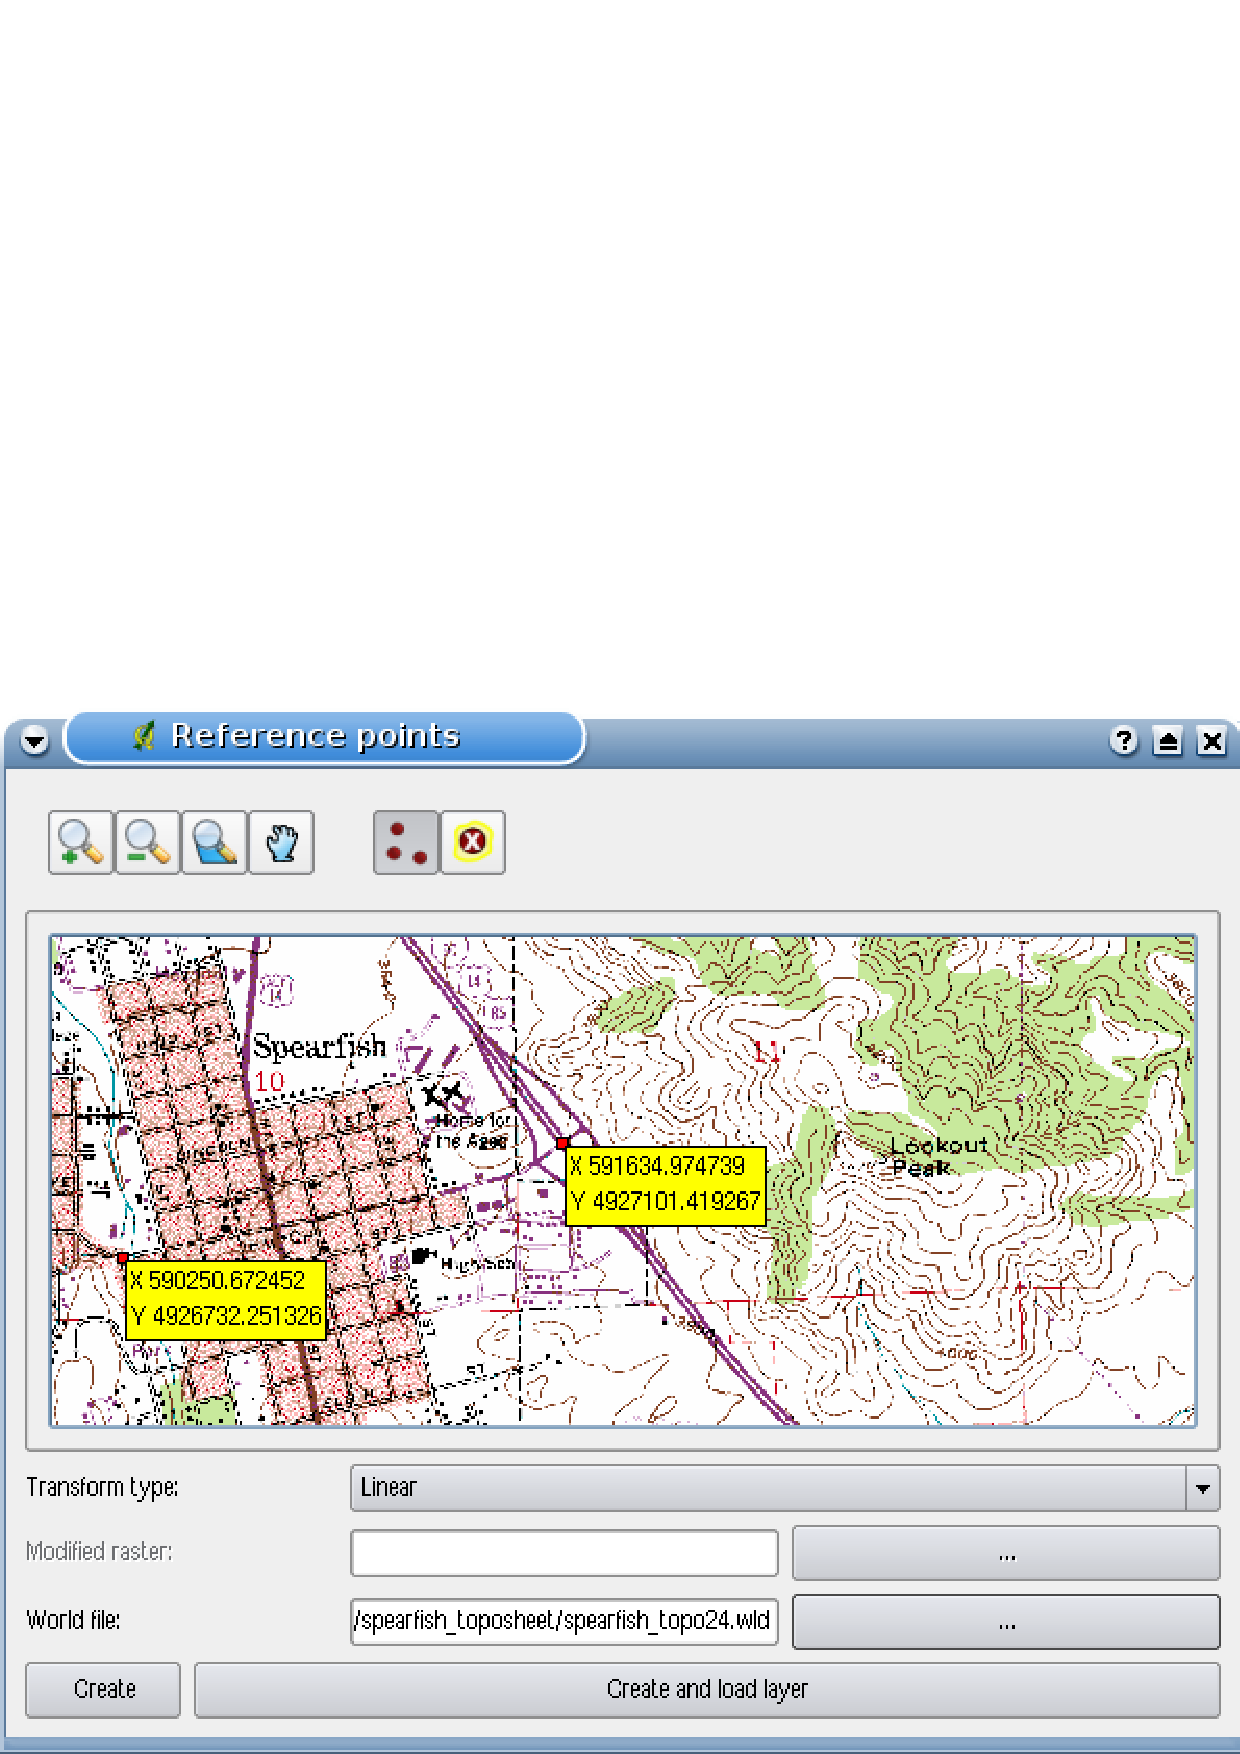
\includegraphics[clip=true,width=9cm]{choose_points}
%\end{center}
%\end{figure}

\begin{figure}[ht]
\begin{center}
  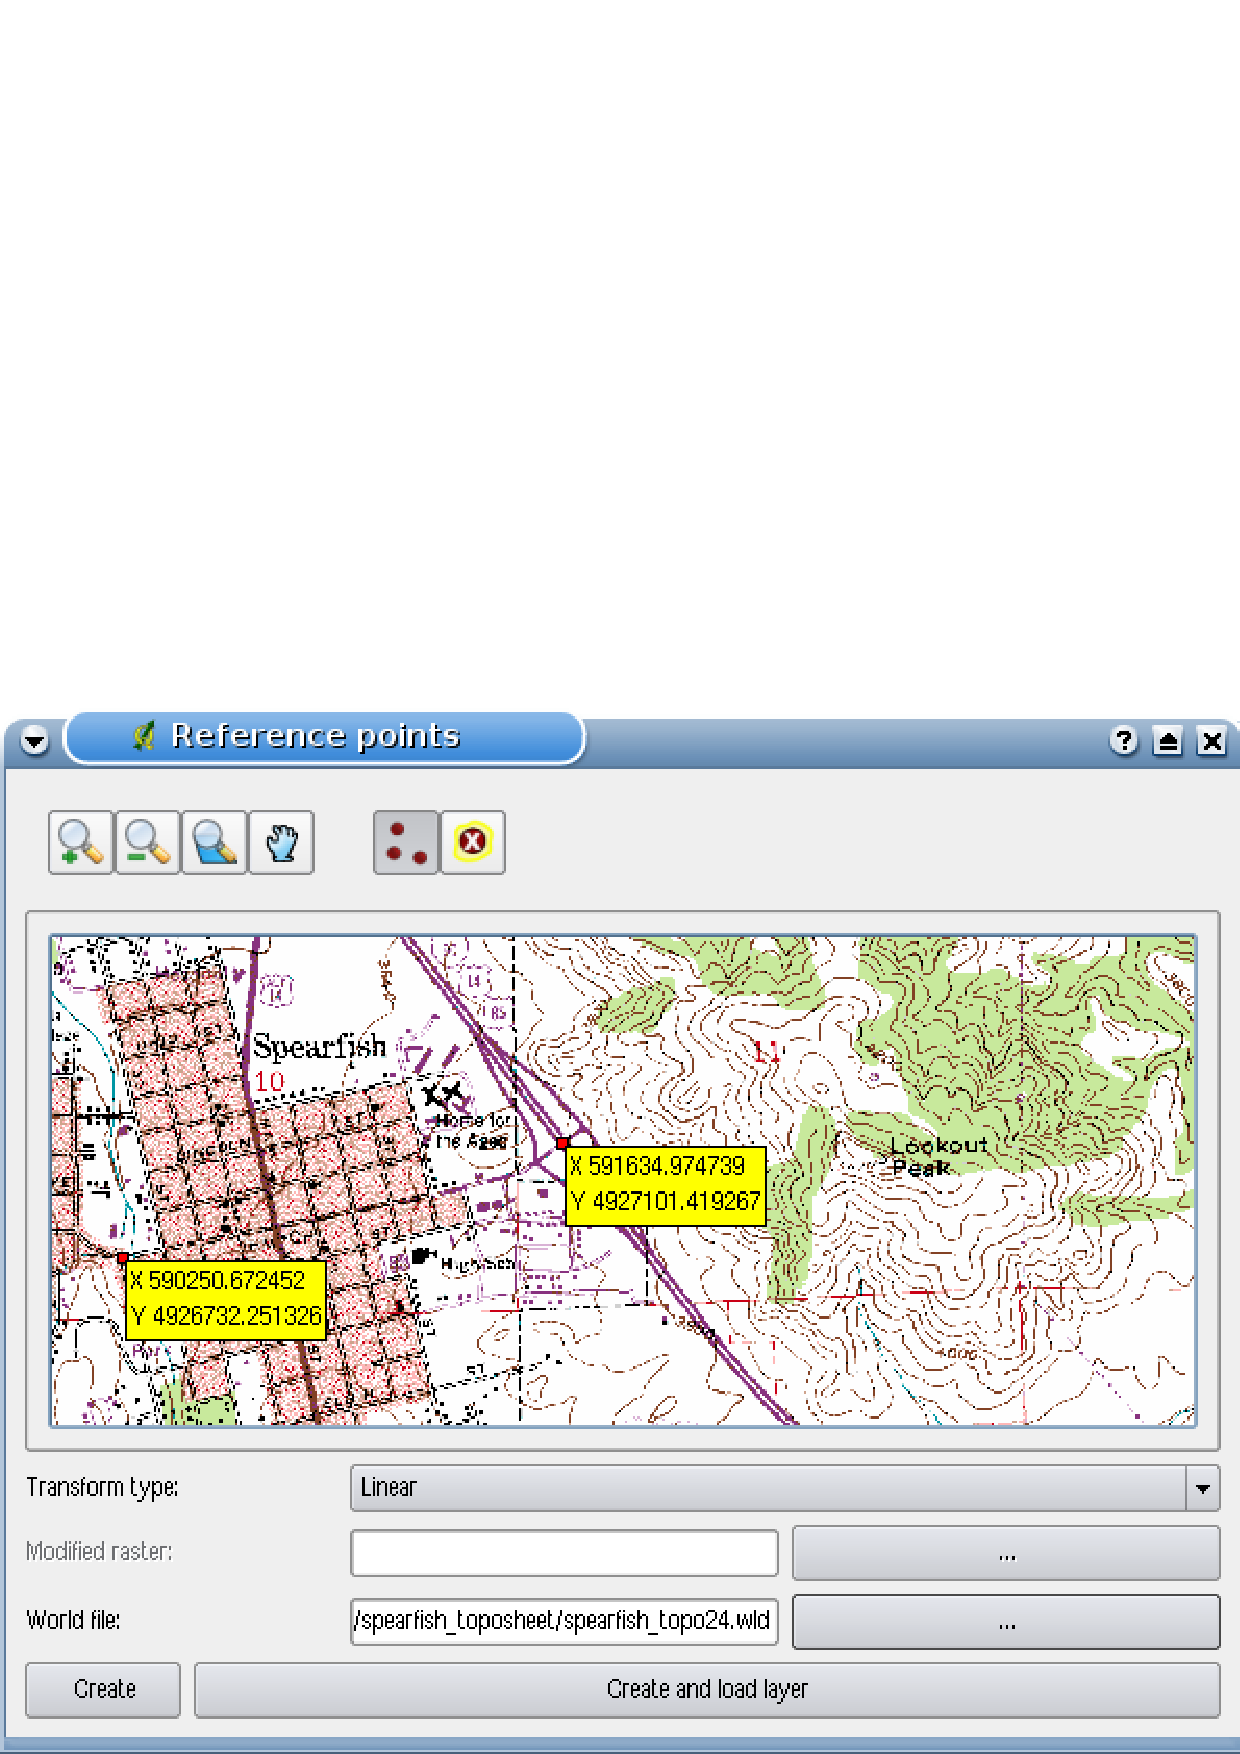
\includegraphics[clip=true,width=9cm]{choose_points}
  \caption{Ajout de points à l'image raster \nixcaption}\label{fig:choose_points}
\end{center}
\end{figure}

%The points that are added to the map will be stored in a separate text file ([filename].points) which is stored together with the raster image. This allows us to reopen the Georeferencer plugin at a later date and add new points or delete existing ones to optimize the result. The points file contains values of the form: mapX, mapY, pixelX, pixelY. You can also \button{Load GCPs} and \button{Save GCPs} to different directories if you like.

Les points qui sont ajoutés sur la carte sont enregistrés dans un fichier texte distinct ([nomduichier].points) qui est stocké avec le fichier raster. Il permet de rouvrir l'extension à une date ultérieure et de rajouter de nouveaux points ou d'effacer ceux existants pour améliorer le résultat. Le fichier de  point contient les valeurs suivantes : mapX, mapY, pixelX, pixelY. Vous pouvez aussi faire \button{Charger GCPs} and \button{Enregistrer GCPs} dans des répertoires différents si vous le désirez.

%\minisec{Choosing the transformation}\label{georeferencer_transformation}
\minisec{Choosing the transformation}\label{georeferencer_transformation}

%After you have added your GCPs to the raster image, you need to select the transformation type for the georeferencing process. Depending on how many ground control point you have captured, you may want to use different transformation algorithms. Choice of transformation algorithm is also dependent on the type and quality of input data and the amount of geometric distortion that you are willing to introduce to final result.

Après avoir ajouté vos points de contrôle, vous devez sélectionner la méthode de transformation qui sera utilisée pour le géoréférencement. Selon le nombre de points que vous avez recueilli, vous devrez utiliser l'algorithme le plus adapté. Le choix de cet algorithme dépend aussi du type et de la qualité des données et de la somme des distorsions géométriques que vous estimerez acceptable pour produire le résultat final.

%Currently, several algorithms are available:

Actuellement plusieurs algorithmes sont disponibles :

%\begin{enumerate}
%\item Linear
%\item Helmert
%\item Polynomial 1
%\item Polynomial 2
%\item Polynomial 3
%\item Thin plate spline (TPS)
%\end{enumerate}

\begin{enumerate}
\item Linéaire
\item Helmert
\item Polynomiale de 1\ier ordre
\item Polynomiale de 2\ieme ordre
\item Polynomiale de 3\ieme ordre
\item Thin plate spline (TPS)
\end{enumerate}

%\begin{itemize}
%\item The Linear algorithm is used to create a world-file, and is different from the other algorithms, as it does not actually transform the raster. This algorithm likely won't be sufficient if you are dealing with scanned material.
%\item The Helmert transformation performs simple scaling and rotation transformations. 
%\item The Polynomial algorithms are among the most widely used algorithms for georeferencing, and each one differs by the degree of distortion introduced to match source and destination ground control points. The most widely used polynomial algorithm is the second order polynomial transformation, which allows some curvature. First order polynomial transformation (affine) preserves colliniarity and allows scaling, translation and rotation only.
%\item The Thin plate spline (TPS) algorithm is a more modern georeferencing method, which is able to introduce local deformations in the data. This algorithm is useful when very low quality originals are being georeferenced.
%\end{itemize}

\begin{itemize}[label=--]
\item L'algorithme linéaire est utilisé pour créer un fichier world et diffère des autres dans le fait qu'il ne transforme pas vraiment le raster. Il ne sera sans doute pas satisfaisant si vous avez à faire à des travaux scannés.
\item La transformation de Helmert réalise une simple mise à l'échelle et une rotation.
\item Les algorithmes polynomiaux sont ceux les plus utilisés pour le géoréfrencement, chacun diffère des autres par le degré de distrotion introduit dans la tentative de de se rapprocher de la source originelle et des points de contrôle. Le plus courant est celui de deuxième ordre qui permet de courber l'image. La transformation de premier ordre (affine) préserve l'aspect et permet seulement la mise à l'échelle, le déplacement et la rotation.
\item L'algorithme de Thin plate spline (TPS)  est une méthode plus moderne qui est capable  d'introduire des déformations sur des secteurs précis de l'image. Il est très pratique quand des sources de faible qualité sont utilisées.
\end{itemize}

%\minisec{Running the transformation}\label{georeferencer_running}
\minisec{Lancer la transformation}\label{georeferencer_running}

%\begin{enumerate}
%\item When the GCPs have been collected, and the transformation has been chosen, press either \button{Create} to create a new raster or \button{Create and load layer} to automatically add the new raster to the layer list.
%\item A warning message will appear that will inform you that a new raster (in GeoTIFF format) will be created.
%\item After hitting OK, you will also be asked to choose a resampling method. There are three methods available:
\begin{enumerate}
\item Quand les GCPs ont été collectés et la transformation choisie, pressez soit \button{Créer} pour créer un nouveau raster ou \button{Créer et charger la couche} tpour ajouter automatiquement le nouveau raster à la liste des couches.
\item Un message d'avertissement s'affiche pour vous informer qu'un nouveau raster (au format GeoTIFF) sera créé.
\item Après avoir cliqué sur OK, il vous sera demandé de choisir une méthode de ré-échantillonna\-ge. Voici les  trois méthodes disponibles :

\begin{enumerate}
\item Au plus proche voisin
\item Linéaire
\item Cubique
\end{enumerate}
\end{enumerate}

%\begin{Tip}\caption{\textsc{Choosing the resampling method}}
%\qgistip{The type of resampling you choose will likely depending on your input data and the ultimate objective of the exercise. If you don't want to change statistics of the image, you might want to choose Nearest neighbour, whereas a Cubic resampling will likely provide a more smoothed result.}
%\end{Tip}
\begin{Tip}\caption{\textsc{Choosing the resampling method}}
Le type de ré-échantillonnage à retenir dépendra de votre donnée en entrée et de l'objectif de l'exercice. Si vous ne voulez pas changer les statistiques de l'image, vous devriez sélectionner la méthode du plus proche voisin tandis que le ré-échantillonnage cubique produira un résultat plus lisse.
\end{Tip}